\section{Theory}
\label{sec:theory}
\paragraph{radioactivity} was discovered by Henri Becquerel and the outcome of his experiments
were presented in 1896 at the conference of the French Academy (see \cite{konya2012nuclear} for 
more detailed information about the following paragraph). 
When studying 
fluorescence he was following a family tradition, since already his father and his grandfather had been
working in this field. At the very time before the discovery he was studying the florescent properties
of potassium uranyl sulfate. Wilhelm Röntgen had shown that X-rays can be indicated by phosphorescent light
emitted by the wall of a X-ray tube; following from there Henri was curious if the reverse process was also
possible: Emission of X-rays through phosphorescent light. In order to examine this idea he exposed
the potassium uranyl sulfate to sunlight, wrapped it in black paper after and placed it on a photograpic plate.
The result was the detection of X-rays. After repeating the experiment without sunlight, he observed the 
same X-rays. He concluded that the blackening of the photographic plate was not caused by fluorescence
induced by sunlight, but rather by an intrinsic property of the uranium salt, which was called Becquerel rays
after. We will give an overview of the theory of radioactive phenomena in general and come back later
to the scope of our experiment.
\subsection{Short introduction to nuclear physics}
\paragraph{In order to understand}
the notions of radioactie decay and half life, we
give a short introduction into nuclear physics following \cite{martin2006nuclear}
In the following, let $Z$ be the atomic number, $N$ the number of neutrons and $A$ the number of nuclei, also
called nucleon number. Thus, $A = Z + N$. The electric charge of the nucleus in the ground state is $+Z e$.
It is common to describe the so called \emph{nuclides} with $_{Z}^{A}\textrm{Y}$.\\
The forces binding the nuclei contribute to the total mass of an atom in terms of the 
binding energy $\Delta E = \Delta M c^2$:
\begin{equation}
\Delta M = M_{tot.} - Z(M_p + M_e) - N M_n \, .
\end{equation}
We used the proton, electron and neutron masses $M_p$, $M_e$ and $M_n$ 
(see figure~\ref{fig:bindingenergy}).
\begin{figure}[htpb]
    \centering
    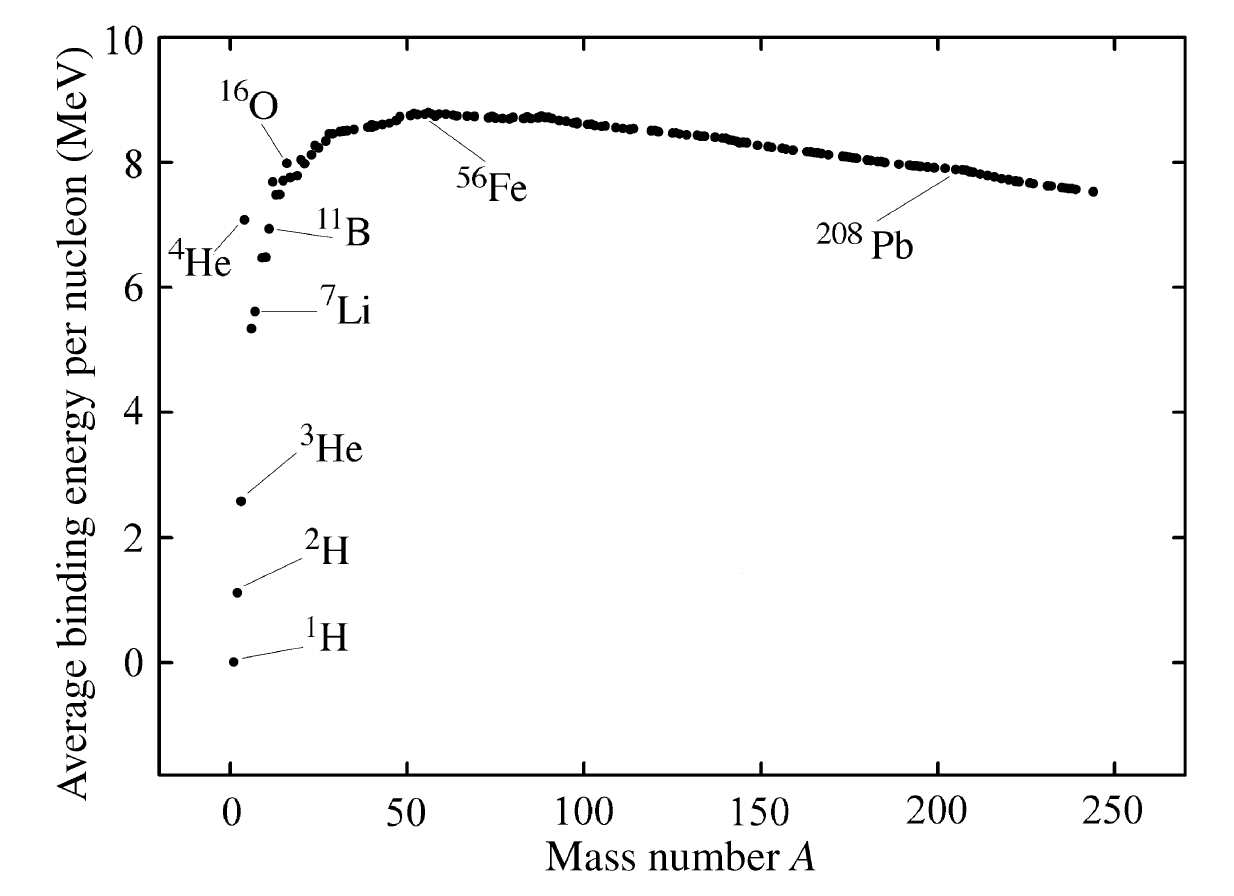
\includegraphics[width=0.8\linewidth]{figures/bindingenergy}
    \caption{Binding energies for nuclei that are stable or long-lived \cite{Hooshyar}.}
    \label{fig:bindingenergy}
\end{figure}
If we look at the distribution of stable nuclei we notice
that they occur only in a very narrow band. All other nuclei are unstable and decay spontaneously.
The decay is characerized by a \emph{decay constant} $\lambda$, which is related to the activity $\mathcal{A}$
by 
\begin{equation}\label{eq:decay}
    \mathcal{A} = -\frac{\partial N}{\partial t} = \lambda N 
\end{equation}
where the activity $\mathcal{A}$ is typically given in Bequerel: $1 \textrm{Bq}= \textrm{decay}\cdot s^{-1}$.
A solution to the differential equation \eqref{eq:decay} is
\begin{equation}
    \mathcal{A}(t) = \lambda N_0 \exp(-\lambda t) \, ,
\end{equation}
with the initial condition $N_0 := N(t=t_0)$. 
The probability of an atom to decay within time $t$ is thus
\begin{equation}
    \mathcal{P}(t) = \int_{0}^{t}\lambda \exp(-\lambda t')\mathrm{d}t' = 1 -  \exp(-\lambda t)  \quad
    \textrm{with} \quad \int_{0}^{\infty}\lambda \exp(-\lambda t')\mathrm{d}t' = 1 \, .
\end{equation}
The probability density is accordingly $f(t) = \lambda \exp(-\lambda t)$. 
Hence, we can calculate the expectation value of a random variable $t$ within the probability space
$\Omega$ with the measure  $\mathcal{P}$:
\begin{equation}
    \tau := E[t] = \int_{0}^{\infty} t \lambda \exp(-\lambda t) \mathrm{d}t 
    =\lim_{t \rightarrow \infty}\left[ \frac{exp(-\lambda t) (1-\lambda t) - 1 }{\lambda} \right] 
= \frac{1}{\lambda}
\end{equation}
The half-life $t_{1/2}$ is obviously connected by $t_{1/2}= -\mathrm{log}(2)/ \lambda = - \tau \mathrm{log}(2)$.

\subsection{Modes of radioactive decay}
\paragraph{Radioactivity has been}
experimentally observed since the end of the 19th century, 
starting with the experiments of Henri Becquerel (1896) as already mentioned, when the atom was still seen 
either within the 'plum pudding model', and later, after the experiments performed by 
Rutherford et.~al. in 1911, a 'planetary model'. Rutherford coined the terms still in 
use today to describe various types of radioactive decay, using the greek letters 
$\alpha$, $\beta$ and $\gamma$. A more refined but not complete overview is 
given by the following.~ \cite{martin2006nuclear}
The mass and atomic numbers of the daughter nuclei ($A'$ and $Z'$, respectively) 
is given in terms of $A$ and $Z$ corresponding to the parent nucleus. 
\begin{description}
    \item [Decay involving the emission of nuclei:] Changing both $A$ and $Z$.
        \begin{itemize}
            \item
                \textbf{$\alpha$-decay:} a $~_2^4$He particle is emitted, the daughter nucleus 
                has a mass number of $A' = A - 4$ and atomic number $Z' = Z - 2$. Example:
                \begin{equation}
                    \mathrm{~^{238}_{92}U}\rightarrow\mathrm{~^{234}_{90}Th} + \mathrm{~^{4}_{2}He} 
                \end{equation}
            \item
                \textbf{Spontaneous fission:} parent nucleus breaks up into two daughter nuclei \emph{without}
                external action. This only occurs in very heavy nuclei. $\mathrm{~^{238}_{92}U}$ can be
                used as an example in this case, as well:
                \begin{equation}
                    \mathrm{~^{238}_{92}U}\rightarrow\mathrm{~^{145}_{57}La} + \mathrm{~^{90}_{35}Br} + 3n  \, .
                \end{equation}
                Instead of breaking into two parts of equal size, the most probable cases yield daughter 
                nuclei differing by approximately 45 in mass number -- a question that remains to be solved 
                until today.
        \end{itemize}
    \item [$\beta$ decay:]
        This form of radioactive decay is observed in atoms of lower mass also. 
        It conserves mass number $A$. Furthermore the $\beta$ decay is characterized by 
        continuos spectrum of energies, since the energy will we redistributed according to
        elastic scattering theory between the electron and the neutrino.
        \begin{itemize}
            \item
                \textbf{$\beta^-$ decay:} conversion of a neutron into a proton with emission of electron and 
                electron antineutrino, raising the atomic number $Z$ by one:
                \begin{equation}
                    {}^{1}_{0} \mathrm {n} \to {}^{1}_{1} \mathrm {p} + \mathrm{e}^{-} + \overline{\nu}_e 
                \end{equation}
            \item
                \textbf{$\beta^+$ decay:} conversion of a proton into a neutron with emission of positron and 
                electron neutrino, reducing the atomic number $Z$ by one:
                \begin{equation}
                    {}^{1}_{0} \mathrm {p} \to {}^{1}_{1} \mathrm {n} + \mathrm{e}^{+} + \nu_e 
                \end{equation}
            \item
                \textbf{Electron capture (EC):} an electron of one of the inner orbitals is 'captured', transforming a proton 
                into a neutron under emission of an electron neutrino
                \begin{equation}
                    {}^{1}_{0} \mathrm {p} + \mathrm{e}^{+} \to {}^{1}_{1} \mathrm {n} + \nu_e 
                \end{equation}
                In most cases, the electron stems from the K-orbital. The daugther nucleus is left in 
                an unstable excited state, like in the case of the $^{40}$K used in the experiment. 
                Figuratively, the hole in the lower shell produced by the $e^-$-capture is successively 
                passed to the outer ones under emission of characteristic $\gamma$-rays. The
                electron capture will also play a role in our experiment, therefore we will
                have to modify the expression for the activity of the observed $\beta$ decay (see equation
                \eqref{eq:EC} for the modification).

        \end{itemize}
    \item [Transition between states of the same nucleus:] 
        A nucleus in an excited state decays into a state of 
        lower energy without changing $A$ and $Z$.
        \begin{itemize}
            \item
                \textbf{Isomeric transition:} The energy is transfrerred to a photon. This is the process to be observed 
                in the experiment. 
            \item
                \textbf{Internal conversion:} Succession transfer of energy to an elctron of the outer orbital, 
                which is then ejected. The resulting excited state is lowered by emission of characteristic 
                x-rays or a so-called \emph{Auger electron}. 
        \end{itemize}
\end{description}



\subsection{Ionization detector}
\label{subsec:detector}
The detection of charged particles can be realized with various different concepts, most of them based on
the concept of the Photoelectric effect, Compton effect or, as in our case, ionization. Our detector is a
kind of Geiger–Müller counter, which yields electric pulses proportional to the incident charged particles.
We apply a electric field in order to attract positive ions created by interaction with the charged particles.
A condensator reacts upon these pulses by a potential difference \cite{staatsexamen}. \\
The change of potential at the condensator
creates a flow, which can be tracked down with the electronic devices. By identifying pulses of a certain
energy with single particles, we can count the single pulses. Since the ionization process is based upon the
decomposition of molecules, we have provide a constant exchange of the gas to be ionized; we will use
methane in our experiment, since it is cheap and effective enough for our purposes\cite{staatsexamen}. \\
Our device can detect particles in all direction ($2\pi$ setup) and is hence cylindric.
The detector is designed for specific domain; below and above this domain we will have nonlinear effects,
which will be described in the following:
\begin{enumerate}
\item If the applied voltage is too low or zero, the potential difference at the condensator will be maximally
exactly proportional to the effect of the charged particles, but there is no amplification. Therefore the
signal will be too low for us to distinguish it from random noise or fluctuations. Below a certain 
applied voltage we will not even create any ions, since we need to surpass at least (using the Bohr model) the
binding energy of the electrons.
\item In the regime above the first one each ionization which was created by a charged particle in the first part will be further
amplified by the applied voltage, leading to a knock-on effect of ionization. Therefore the detected signal
will be higher by orders of magnitude and therefore distinguishable from noise.
\item Above the regime denoted as propotionality regime we enter a nonlinear domain. First, the finite 
ionizability will lead to a saturation of any further amplification. After further increasing of the voltage
the energy surplus can lead to a phase transition of the gas into plasma, which is dominated by strong
fluctuations distorting the detected signal.
\end{enumerate}
As it turns out we will try to stay in the second regime, maximizing the signal. Furthermore we have to
consider the different shapes of our signal depending on the applied voltage and the decay mode.
\subsubsection{Plateaus}
\label{subsec:plateaus}
One of our first measurements will be the detection of both $\alpha$ and $\beta$ rays of a uranium preperation.
An important point is that $\alpha$ particles are carrying much more energy than $\beta$ particles, and
have thus a far higher capability to ionize the gas. Hence, we do need less amplification to detect $\alpha$
particles than to detect $\beta$ particles. By applying the concepts about the regimes from the last 
paragraph, we realize that there will be two \textit{plateaus}, depending on the required amplification of
the particles in order to ionize the gas up to the second regime (see our measurements for a visualization
of this rather abstract concept, subsection\ref{subsec:uranium}).
\subsection{Potassium}
\label{subsec:potassium}
Potassium was discovered in 1807 by Davy with the at that time new method of electrolysis. The metal
is the seventh most abundant and makes up about 2.4\% by weight of the Earth's crust \cite{haynes}.
The emission of $\beta$-rays is continuos due to the absorption when
passing through matter. Following \cite{ver} we will observe the following
counting rate
\begin{equation}
n(m) = f_B \frac{\Omega}{4 \pi} A_s \frac{F \rho }{\mu}A \left (1 - \exp \left ( - \frac{\mu}{F \rho}m \right ) \right )
\label{eq:potassium}
\end{equation}
Where we defined the following coefficients:
\begin{itemize}
\item[] $A_s = A/ m$... specific activity of the preperation  
\item[] $\mu$ ... extinction coefficient  of the $\beta$ decay 
\item[] $\Omega = 2 \pi$... solid angle
\item[] $f_B\approx 1.29$ ... backscattering coefficient 
\end{itemize}
We will use a least squares optimization in order to estimate the coefficients for the equation:
\begin{equation}
n(m) = a ( 1 - e^{-bm})
\end{equation}
such that we can identify the parameters
\begin{align}
a &\equiv  f_B \frac{\Omega}{4 \pi} A_s \frac{F \rho }{\mu}A  \label{eq:a}\\ 
b &\equiv \frac{\mu}{F \rho} \label{eq:b}
\end{align}
For calculating the half life time, we use $T_{1/2} = \frac{\mathrm{log}(2)}{\lambda}$. Unfortunatelly,
we cannot use the $\lambda$ directly for the activity, since the activity does not resample the real activity, but
the due to electron capture reduced activity. We can use the following estimation \cite{ver}:
\begin{equation}
\lambda = \lambda_{\beta} + \lambda_{EC} = \lambda_{\beta} + \frac{0.1072}{0.8928}\lambda_{\beta} = 1.12 \lambda_{\beta}
\label{eq:EC}
\end{equation}
which let us arrive at the following result
\begin{align}
A = N \lambda = 1.12 \cdot N\lambda_\beta= N \tau ^{-1} \Leftrightarrow  T_{1/2} = \frac{N \mathrm{log}(2)}{1.12 \cdot A}.
\label{eq:As}
\end{align}
Additionally to that, we are using the specific Activity $A_s = A / m$ with the molar mass $m$. Since we are not using
pure $^{40}\textrm{K}$ cores but KCl, we have to take the relative occurence of those in our sample into consideration by
\begin{equation}
N = \frac{h_{rel} m N_A}{m_{\mathrm{KCl}}}
\end{equation}
with the Number of $^{40}\textrm{K}$ cores, the relative mass ratio of $^{40}\textrm{K}$ in natural kalium $h_{rel} = 1.18 \cdot 10^{-4}$,
the Avogadro constant $N_A$ and the molar mass $m_{\mathrm{KCl}}$ of KCl.
Plugging in equation \eqref{eq:a}, \eqref{eq:As} and in the end \eqref{eq:b} we get to the final result (where the factor $m$ chancels)
\begin{equation}
A_s = \frac{A}{m} =  \frac{4 \pi a \mu}{\Omega f_B F \rho} \Leftrightarrow T_{1/2} = \frac{N \Omega f_B F \rho \mathrm{log}(2)}{1.12 \cdot 4 \pi m a \mu} 
= \frac{N \Omega f_B \mathrm{log}(2)}{1.12 \cdot 4 \pi m a b} = \frac{N_A h_{rel}\Omega f_B \mathrm{log}(2)}{1.12 \cdot 4 \pi a b m_{\mathrm{KCl}}}
\end{equation}
At this point we use $f_B=1.29$, $\Omega = 2 \pi$ and $\eta = [3.80 \pm 0.06]\cdot 10^{17}$ counts/g (where estimated the errors of the constants to be of the 
same order of magnitude as the last digit) to arrive at
\begin{equation}
T_{1/2} = \frac{\eta}{a b} 
\label{eq:pot_final}
\end{equation}
\subsection{Samarium}
\label{subsec:samarium_theory}
Samarium was discovered spectroscopically by its sharp absorption lines in 1879
by Lecoq de Boisbaudran \cite{haynes}
in the mineral samarskite, which is named in honor of a Russian minie offical, Colonel Samarski.
Natural samarium isa mixture of seven isotopes, three of which are unstable but have long half-lives.
We will use the detection of $\alpha$ rays for estimating the half life period of samarium. 
The emission depends to a great deal on the surface of the emitting object.
Following \cite{ver} the rate $n$ of samarium can be calculated with
\begin{equation}
n = A_v \frac{F}{4} R_{Sm_2O_3}
\label{eq:range2}
\end{equation}
where we introduced the Activity per Volume $A_v = A/V$, the range $R_{Sm_2O_3}$ and the Surface area $F$.
Since it is not always possible to conduct experiments for all possible incident particles and materials, we
can estimate the range with the \textbf{Bragg-Kleemann rule} \cite{knoll2000radiation}, if we know
the range for another material:
\begin{equation}
    \frac{R_1}{R_0} = \frac{\rho_0 \sqrt{m_{eff,1}}}{\rho_1 \sqrt{m_{eff,0}}} 
    \label{eq:range}
\end{equation}
where we have two materials and the respective radii $R$, densities $\rho$ and atomic weights $A$. 
The effective mass molar mass $m_A$ has to be concluded from the single weights of the atoms and the relative densities of these with
\footnote{%
    We have to raise strong doubts about the academic integrity the source \cite{ver}, since no source for equation~\ref{eq:masses} was given.
    Probably it was taken from \cite{staatsexamen}, but even there we cannot find any reference or source for the formula, which even more violates our
    understanding about scientific practice: This formula is neither generally valid nor trivial. 
    After some research we found it within the book \cite{knoll2000radiation}. The main argument is the following: A \textit{linear stopping power S} for
    charged particles in a given absorber is defined by the differential energy loss for that particle within the material, divided by the corresponding
    differential path length:
    \begin{equation}
    S = - \frac{\del E}{\del x} = \frac{4 \pi e^4 z^2}{m_e v^2} N B 
    \end{equation}
    where the last step is the famous, but classical derived Bethe formula with velocitiy $v$ and charge $z$ of the particle, Number density $N$ and atomic number $Z$
    of the adsorber atoms and the electron rest mass $m_e$. The paramter $B$ is an expression obtained from integration, dependent on $v$ and average excitation and
    ionization potential of the adsorber. Now we have to implied various assumptions:
    \begin{itemize}
    \item The stopping power per atom of compounds or mixtures is additive (known as \textbf{Bragg-Kleemann rule}).
    \item The particle should be heavy and charged, like alpha particles, in order to interact with matter primarily through coulomb forces
    between their charges
    \item Interactions with nuclei can be neglected, since they happen only rearely and they are not significant in the response of radiation detectors.
    \item The charged particle immediately interacts simultaneously with many electrons, depending on the proximity either to raise the respective electron to
    a higher lying shell within the adsorber (\textit{excitation}) or remove the electron from the atom (\textit{ionization}).
    \end{itemize}
    Going from here the already mentioned \textbf{Bragg-Kleemann rule} can be stated as
    \begin{equation}
    \frac{1}{N_c}\left (\frac{\del E}{\del x} \right )_c = \sum_i P_i  \frac{1}{N_i}\left (\frac{\del E}{\del x} \right )_i.
    \label{eq:masses2}
    \end{equation}
    with the atomic fraction $p_i$ of the ith component in the compound $c$. From equation \eqref{eq:masses2} is now possible with some
    intermediate steps to arrive at \eqref{eq:masses}.
} 
\begin{equation}
\sqrt{m_{eff}} = \sum_i p_i \sqrt{m_{A,i}} .
\label{eq:masses}
\end{equation}

With this formula it is now possible to eliminate the constant $C$, given that we can find the effective mass density for another
material. For instance, air approximately consists of nitrogen, oxygen and argon: 
\begin{equation}
\sqrt{m_{\mathrm{eff,air}}} =p_{\mathrm{N}}\sqrt{m_{\mathrm{N}}} +p_{\mathrm{O}} \sqrt{m_{\mathrm{O}}} +p_{\mathrm{Ar}} \sqrt{m_{\mathrm{Ar}}}
\end{equation}
with the probabilites \cite{ver} and the atomic masses \cite{haynes} in table~\ref{tab:air}.
\begin{table}
\caption{Atomic fractions $p$ and the respective atomic masses $m$ for air.}
\centering
\begin{tabular}{ll}
    \cellcolor{tabcolor} $p_{\mathrm{N}}$    &$0.75518 \pm 0.00001$ \\
    \cellcolor{tabcolor} $p_{\mathrm{O}} $   &$0.23135 \pm 0.00001$\\
    \cellcolor{tabcolor} $p_{\mathrm{Ar}}$   &$0.01288 \pm 0.00001$
\end{tabular}
\begin{tabular}{ll} 
    \cellcolor{tabcolor} $m_{\mathrm{N}}  $ & $[14.0067 \pm 0.0002] u $ \\
    \cellcolor{tabcolor} $m_{\mathrm{O}}  $ & $ [15.9994 \pm 0.0003] u$  \\
    \cellcolor{tabcolor} $m_{\mathrm{Ar}} $ & $ [39.948 \quad \pm 0.001] u $
\end{tabular}
\label{tab:air}
\end{table}
As result we arrive at the effective mass  $m_{\mathrm{eff,air}} = [14.6926\pm0.0007]u$. \\
we have to calculate the effective mass for samarium oxide $Sm_2O_3$ in order to conclude the range:
\begin{equation}
\sqrt{m_{\mathrm{eff,Sm_2O_3}}} =p_{\mathrm{Sm}}\sqrt{m_{\mathrm{Sm}}} +p_{\mathrm{O_3}} \sqrt{m_{\mathrm{O_3}}} 
\end{equation}
with the probabilites\footnote{%
We calculated the probabilites with the approximation\cite{staatsexamen}, 
that the relative probability is proportional
to the number of atoms times the molecular mass: $p_{\mathrm{Sm_2}} = \frac{2 m_{Sm}}{2m_{Sm} + 3m_{O}}$ and
$p_{\mathrm{O_3}} = \frac{3 m_{O_3}}{2m_{Sm} + 3m_{O}}$.
}
and masses \cite{haynes} in table~\ref{tab:sm2o3} we
arrive at $m_{\mathrm{eff},Sm_2O_3}[123.763\pm0.009]u$.
\begin{table}
\centering
\caption{Atomic fractions $p$ and the respective atomic masses $m$ for $Sm_2O_3$.}
\begin{tabular}{ll}
\begin{tabular}{ll}
    \cellcolor{tabcolor}  $p_{\mathrm{Sm_2}}$       &$0.86235\pm0.00001$ \\
     \cellcolor{tabcolor} $p_{\mathrm{O_3}} $   &$0.13764\pm0.00001$ \\
\end{tabular}
&
\begin{tabular}{ll} 
    \cellcolor{tabcolor} $m_{\mathrm{Sm}}  $ & $[150.36 \pm 0.01] u $ \\
    \cellcolor{tabcolor} $m_{\mathrm{O}}  $ & $ [16.000\quad \pm 0.001] u$  \\
\end{tabular}
\end{tabular}
\label{tab:sm2o3}
\end{table}
At this point we can use equation \eqref{eq:range}, by implying the densities\footnote{%
These rely very sensitive on the pressure and Temperature, we used $T = 293^{\circ}K$ and $P = 101kPa$ 
(standard conditions) in the further calculations}\footnote{%
    The density of samarium(III)oxide is different to the
    value given in wikipedia.org and wolframalpha.com, which is $\rho_{Sm_2O_3} = [7.6 \pm 0.1] \mathrm{g/cm}^3$,
    because we used \cite{haynes}, which we consider to be a more reliable source, since the other
    two sources rely to some extent upon an older version of \cite{haynes}.
}\\
$\rho_{air} = [0.001184 \pm 0.0001] \mathrm{g/cm}^3$ and
$\rho_{Sm_2O_3} = [7.6 \pm 0.1] \mathrm{g/cm}^3$ \\ and the range of $\alpha$ rays in air
$R_{\mathrm{air}} = [1.13\pm0.12]$cm (\footnote{%
We used this value from \cite{ver}, because it was not possible to determine the value in a better
fashion, because the range of $\alpha$ rays depends strongly on their energy, which ranges in the $\alpha$ decay
from 2 - 10 MeV \cite{konya2012nuclear} (in our case, the energy is given by $E_\alpha = [2.233 \pm 0.001]MeV$
\cite{staatsexamen}).
Let us assume
we want to determine the range in air, then the range depends on the interaction of the alpha particles with
the orbital electrons of the molecules. The range of the particles is closely approximated
by \cite{cember1996introduction}:
\begin{equation}
R_{\mathrm{air}} =
\begin{cases}
0.56 E_\alpha \qquad \text{ for } E_\alpha < 4 \mathrm{MeV} \\
1.24 E_\alpha - 2.62 \qquad \text{ for } E_\alpha < 4 \mathrm{MeV} 
\end{cases}
\end{equation}
As it can be seen the ranges vary greatly, depending on the energy. Plugging in $E_\alpha$ we get
\begin{equation}
R_{\mathrm{air}} = [1.250\pm0.022] \mathrm{cm}
\end{equation}
Which varies from the value given in \cite{staatsexamen}. However, we
will take their value
\begin{equation}
R_{\mathrm{air}} = [1.13\pm0.12] \mathrm{cm}
\end{equation}
with a greater error in order to account for our previous calculation.
}):
\begin{equation}
    R_{Sm_2O_3} =R_{\mathrm{air}} \frac{\rho_{\mathrm{air}\sqrt{m_{\mathrm{eff,Sm_2O_3}}}}}
    {\rho_{\mathrm{Sm_2O_3}} \sqrt{m_{\mathrm{eff,air}}} } 
    = [5.1 \pm 0.7] \mathrm{\mu m}
\end{equation}





This range seems to be very small compared to the range in air, but one has to consider the much higher density
in $Sm_2O_3$ which contributes to a huge extent to the absorption. \\
The next step is to consider the activity per volume using \eqref{eq:range2}
\begin{equation}
A_v = A \cdot V = A \cdot F \cdot d = \frac{4\cdot n \cdot d}{R_{Sm_2O_3} }.
\end{equation}
with the sample width $d$ and the surface $F$. From here the half life period directly follows with
\begin{equation}
T_{1/2} = \frac{\mathrm{log}(2)N}{A} = \frac{log(2) N R_{Sm_2O_3}F}{4 n \cdot V}.
\label{eq:T12_sam}
\end{equation}

This expression only leaves to estimate the number of $^{147}Sm$ atoms $N$ with
\begin{equation}
    N = p_{\mathrm{^{147}Sm}} \cdot N_{\mathrm{Sm_2O_3}} 
    \qquad \text{ with \cite{haynes} } p_{\mathrm{^{147}Sm}}= [0.1499\pm0.0033]
\end{equation}
(since for the radiation we only
rely on the atoms which are decaying into neodym), hence
\begin{equation}
    N = 2 \cdot p_{\mathrm{^{147}Sm}} \cdot N_{\mathrm{Sm_2O_3}} 
    = \frac{2 \cdot p_{\mathrm{^{147}Sm}} \cdot N_A m}{m_{\mathrm{Sm_2O_3, mol}}}
    = \frac{2 \cdot p_{\mathrm{^{147}Sm}} \cdot N_A \rho_{\mathrm{Sm_2O_3}} V}{m_{\mathrm{Sm_2O_3, mol}}}
    \label{eq:N}
\end{equation}
with $m_{\mathrm{Sm_2O_3, mol}} = 348.72 \mathrm{g/mol} $ \cite{haynes}. 
Plugging \eqref{eq:N} into \eqref{eq:T12_sam} we arrive at
\begin{equation}
T_{1/2} = \frac{\mathrm{log}(2)p_{\mathrm{^{147}Sm}} 
 N_A \rho_{\mathrm{Sm_2O_3}}R_{Sm_2O_3}F}{2m_{\mathrm{Sm_2O_3, mol}}n } = \zeta \frac{F}{n} 
\label{eq:T12_sam}
\end{equation}
with $\zeta=[3.5\pm0.5]\cdot10^{17} \mathrm{counts \cdot cm^{-2}}$.

In conclusion, we consider this experiment to be quite interesting since we gained deep 
insight into various concepts of nuclear physics and radio chemistry.

In conclusion, we consider this experiment to be quite interesting since we gained deep 
insight into various concepts of nuclear physics and radio chemistry.
